\chapter{Mathematical Modeling}

\addcontentsline{toc}{chapter}{Mathematical Modeling}

A mathematical model is a description of a system using mathematical concepts and language \cite{per5}. A model may help to explain a system and to study the effects of different components, and to make predictions about behavior \cite{per6}. The traditional models of the disease spreading make assumptions (e.g., uniformity of individuals, their continuous uniform mixing at the modeled area) that are not sufficiently accurate \cite{per7}. Considering the great achievements in mathematics and simulation techniques, building the models that give the most realistic outcome is a fully realizable task. Mathematical models can take many forms, including dynamical systems, statistical models, differential equations, or game theoretic models \cite{per7}. Implementation of mathematical models can be done using different methods and techniques including software and programs. This paper discusses building the mathematical model of influenza epidemics using the system dynamics approach. System dynamics is a concept of understanding the behavior of complex systems over time \cite{per1}]. It deals with different parameters affecting the system and measuring the impacts of those variables on systems \cite{per1}]. System dynamics and the programs for it will be described in more detail in further sections.

\begin{figure}
   \centering
	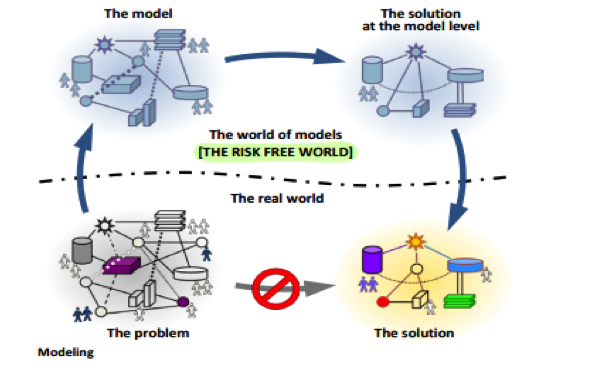
\includegraphics[width=0.9\textwidth]{img/modeling}
	\caption[Clear]{Mathematical modeling benefits visualization}
\end{figure}


Modeling is one of the ways to solve problems that appear in the real world \cite{per9}. In many cases we cannot afford finding the right solutions by experimenting   with real objects:  building, destroying, making changes may be too expensive, dangerous, or just impossible. If this is so, we leave the real world and go up to the world of models, see the Figure 1. We build a model of a real system: its representation in a modeling language. This process assumes abstraction: we throw away the details that are irrelevant to the problem we are trying to solve and keep what we think is important. The model is always less complex than the real system. Having built the model ( or sometimes  even while building the model ) , we  start to explore and understand the structure and behavior of the original system, test how the system will behave under various conditions, play  and compare different scenarios, optimize.  When we find the solution we are looking for, we map that solution back to the real world.

Models are used and successfully applied in different areas starting from logistics to health care systems. Types of modeling include conceptual modeling, analytical modeling and simulation modeling.